%!TEX root = ../paper.tex
\appendix

\section{Fischhoff Prompts}
\label{sec:prompt} 

\textit{We would like to ask you to rate the <risks/benefits> associated with each of the following technologies.}

{\bf Risks:} \textit{Consider all types of risks: the risk of physical harm or death, the risk to others or bystanders, the financial cost of the technology, any distress caused by the technology, what the consequences would be if the technology was misused, any impact on the public, work, or personal life, and other considerations. (e.g. for electricity, consider the risk of electrocution, the pollution caused by coal, the risk that miners need to take to mine the coal, the cost to build the infrastructure to deliver electricity, etc.) Give a global estimate over a long period of time (say, a year) of both intangible and tangible risks.} \\[-.6cm]

\textit{Do not consider the costs or risks associated with these items. It is true, for example, that sometimes swimmers can drown. But evaluating such risks is not your present job. Your job is to assess the gross benefits, not the net benefits which remain after the costs and risks are subtracted out.} \\[-.6cm]

\textit{Please rate the following technologies below with a number. We know that this might be a bit hard to do, but please try to be as accurate as possible, adjusting the numbers until they feel they are right for you. Start with the least risky technology at 10 and assign higher numbers for the more risky technologies. (For instance, a technology rated 14 is half as risky as a technology rated 28.)}

{\bf Benefits:} \textit{Consider all types of benefits: how many jobs are created, how much money is generated directly or indirectly, how much enjoyment is brought to people, how much a contribution is made to the people's health and welfare, what this technology promotes, and so on. (e.g. for swimming, consider the manufacture and sale of swimsuits, the time spent exercising, the social interactions during swimming, and the sport created around the activity.) Give a global estimate over a long period of time (say, a year) of both intangible and tangible benefits.} \\[-.6cm]

\textit{Do not consider the costs or benefits associated with these items. It is true, for example, that electricity also creates a market for home appliances. But evaluating such benefits is not your present job. Your job is to assess the gross risks, not the net risks which remain after the costs and risks are subtracted out.} \\[-.6cm]

\textit{Please rate the following technologies below with a number. We know that this might be a bit hard to do, but please try to be as accurate as possible, adjusting the numbers until they feel they are right for you. Start with the least beneficial technology at 10 and assign higher numbers for the more beneficial technologies. (For instance, a technology rated 34 is twice as beneficial as a technology rated 17.)}

\section{Coding Label Definitions}
\label{sec:coding}

Privacy: ``privacy,'' revealing personal information, spying. \\
Security:  ``security,'' compromise, malware, hacking. \\
GPS tracking: ``location,'' ``GPS,'' being monitored. 

Unaware use: using data without permission or in a different way than understood by user. \\
Unaware collection: collecting data without permission. \\
Unaware access: disclosure of data without permission. \\
False information: inaccurate or maliciously false data.

Health Risk: radiation, cancer, or long-term effects.\\
Safety: distractions causing car crashes or injuries, mugging or violence because of the device, injuries from device malfunctions (battery burns).\\
Discomfort: eye strain, headache, obscured vision, irritation. \\
Financial cost: getting ripped off by buying the device or device accessories, having to buy another device when broken or stolen, financial compromise caused by device. \\
Theft: the device getting stolen. 

Social Impact: dependency, distance from friends and family, changes in decision making, social changes, etc. \\
Social Stigma: judgment, hate, or bystander discomfort.\\ 
Aesthetics: fashion, the device being ugly, mentions of not looking cool/dorky. 

Miscellaneous: odd comments, uncommon concerns. \\
None: ``None,'' no threat, perceiving no big concerns \\
Don't know: ``do not know,'' hinting at confusion \\
Don't care: `` do not care,'' nonchalant answers 



\onecolumn
\section{Full Regression Model from Data Types}
\label{sec:regression}
%\begin{figure*}[t]
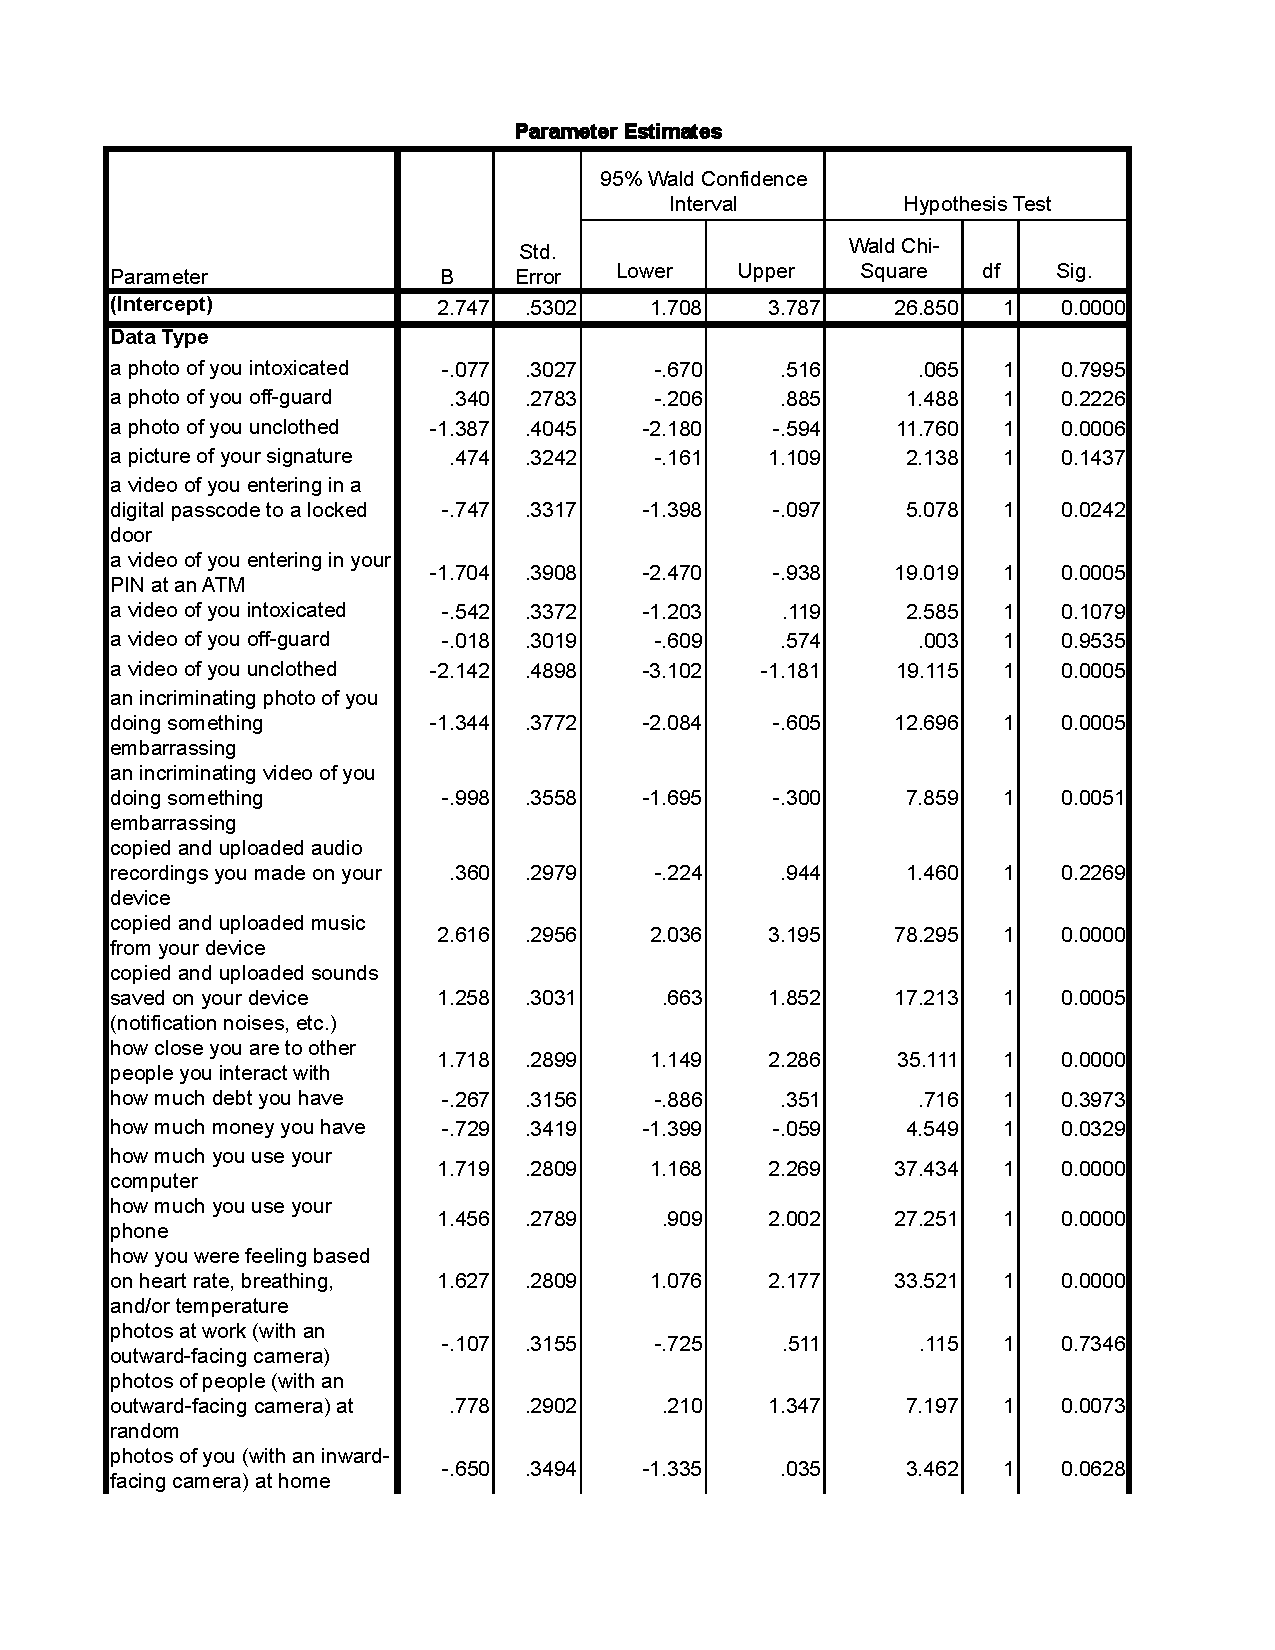
\includegraphics[page=1,scale=0.8]{images/full-model.pdf}
\includepdf[pages=2-3,scale=0.8]{images/full-model.pdf}

%\caption{Full regression model, which includes all 72 data types, recipients, and covariates.}
%\end{figure*}